\chapter{Software Interface}

\section{Driver Interface}
\subsection{Introduction}
The debug interface to the processor is a crucial part in development of applications as well as the development of the processor itself.
Here we attempt to provide a seamless debug interface which is easily extendible and integrable to the FPGA system and new processor cores.
The way the host machine communicates with the processor is by periodically sending and receiving packets of length 64-bits over the PCIe
bus of the host machine to the AXI interconnect on the FPGA system. The following figure shows the debug interface of the processor:-

\begin{figure}[H]
\centering
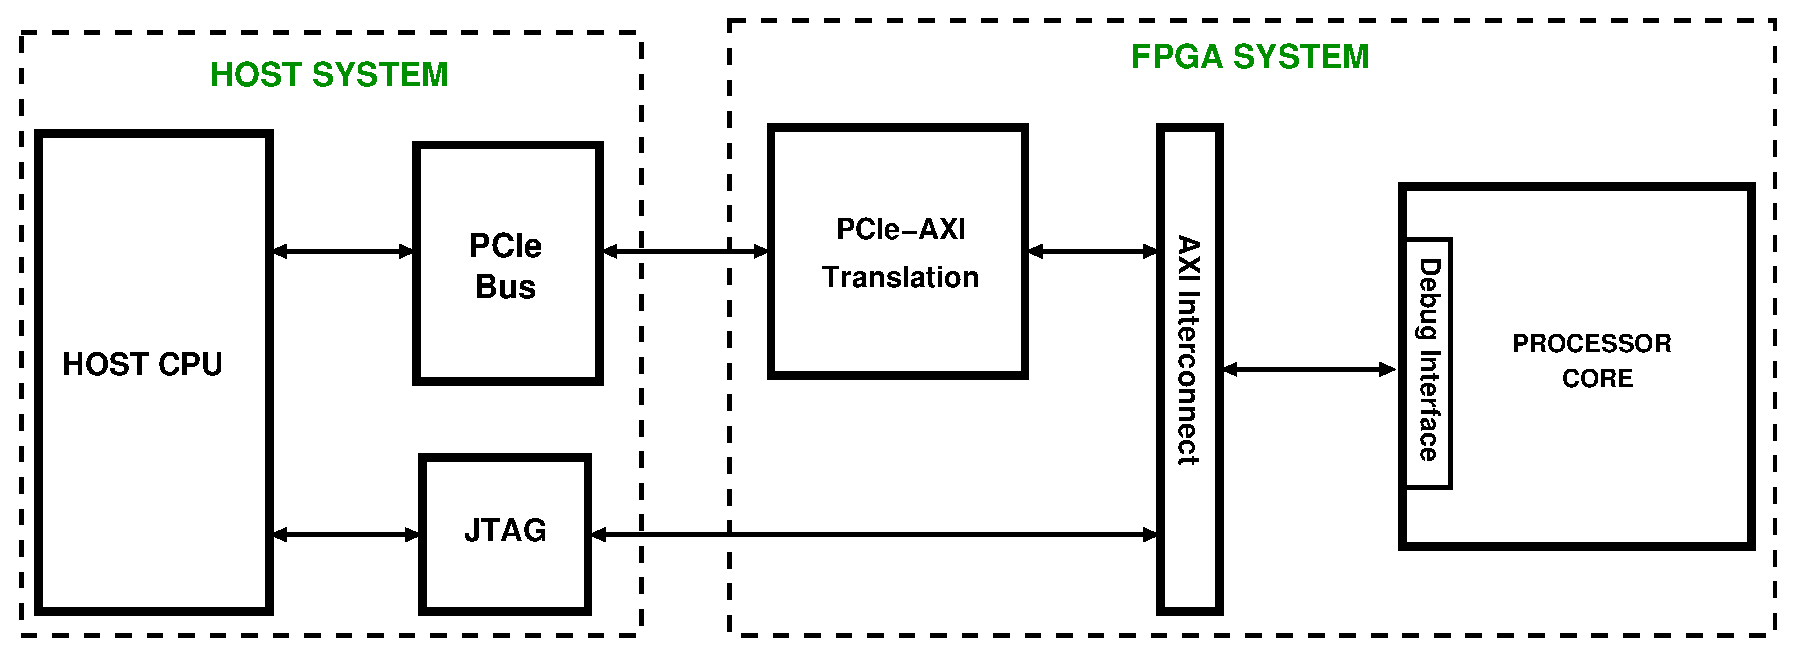
\includegraphics[width=\textwidth]{eps_pdf_sources/ajit_fpga/Debug_Interface/debug_channel_intro}
\caption{Debug channel from host to AJIT}
\end{figure}

\subsection{Testbench for the Driver Interface}
In order to test the FPGA system we run a software testbench on the host machine which controls the processor's mode and reads and writes
the on board memory. The driver API provides lower level function calls to the testbench in order to execute fundamental tasks on the FPGA system.
The testbench builds on this driver and contains a multi-threaded environment with several threads controlling their respective software
pipes which are then collected by the main thread to produce a 64-bit packet which contains the relevant Debug instruction for the processor
to execute. The driver API also aids development of userspace applications which need access to lower level FPGA system routines.

\begin{figure}[H]
\centering
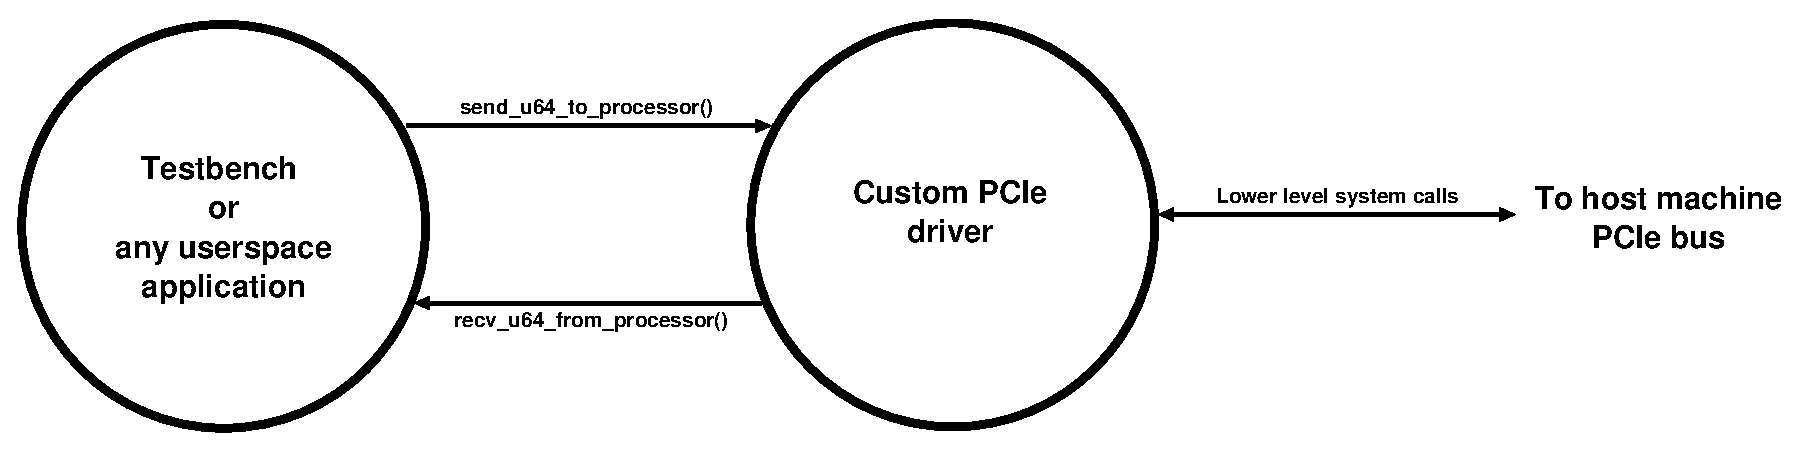
\includegraphics[width=\textwidth]{eps_pdf_sources/ajit_fpga/Software_Interface/testbench_and_application_illustration}
\caption{Driver API in action}
\end{figure}

\begin{figure}[H]
\centering
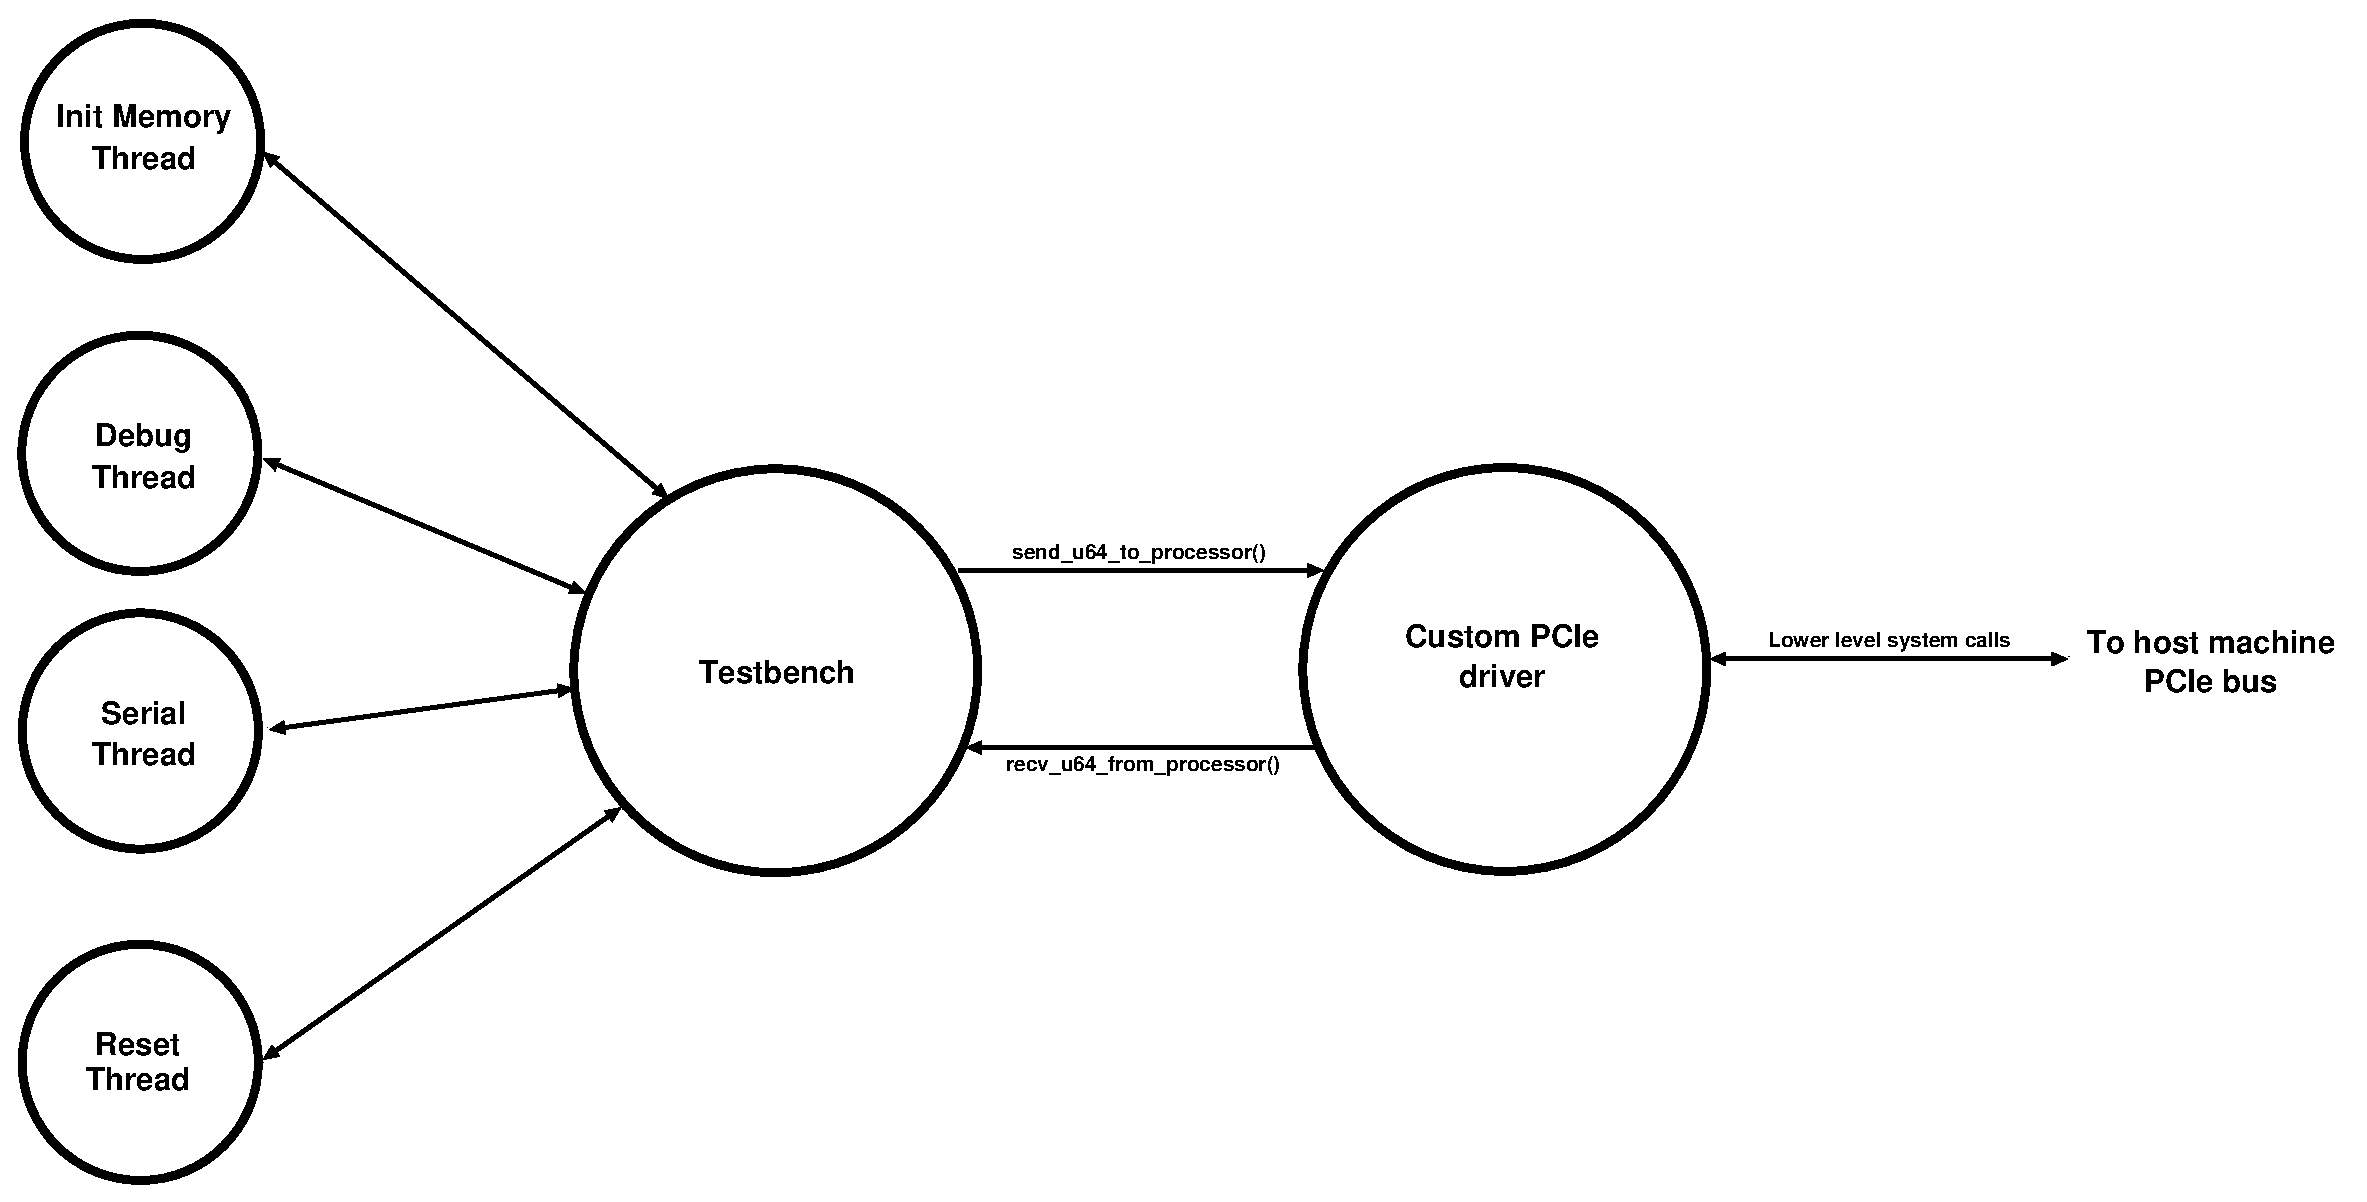
\includegraphics[width=\textwidth]{eps_pdf_sources/ajit_fpga/Software_Interface/testbench_illustration}
\caption{Software Testbench threads}
\end{figure}

%\begin{figure}[H]
%\centering
%\includegraphics[width=\textwidth]{eps_pdf_sources/ajit_fpga/Debug_Interface/aggregator_view}
%\caption{Driver API in action}
%\end{figure}

\section{Driver Interface discussion}

For the previous iteration of already developed software programs for AJIT to be compatible with the new FPGA model we need to keep the
identical call names to the API calls and need to have a Driver API interface which provides the same functions but with non-trivial and
different inherent implementations which is the multiple bars of 128MB one.

\section{Driver API}

The four black boxed functions that the API provides are:

\singlespacing
\scriptsize
\begin{lstlisting}[language=C, caption=Driver API]
void* initialize_axi_link(char* name){
...
}

int close_axi_link(void* fpga_device){
...
}

int write_to_axi_dram(void* fpga_device, uint32_t address, uint32_t write_word){
...
}

int read_from_axi_dram(void* fpga_device, uint32_t address, uint32_t *read_word){
...
}

int recv_u64_from_processor(uint64_t* r_word){
...
}

int send_u64_to_processor(uint64_t* s_word){
...
}
\end{lstlisting}
\normalsize
\doublespacing

\section{Driver development discussion}

Driver infrastructure can be broken down in four simple parts:\\

\verb|initialize_axi_link(...)| \\

As would be evident by the name this function, it initialize the axi link to a fpga device and returns the status of the opened device and prints error message if it
fails to open the device. It initializes an internal data structure specifically created to manipulate fpga devices, allocates memory and
returns a pointer to the created FPGA device.\\

\verb|close_axi_link(...)| \\

As would be evident by the name this function closes an already open fpga device and returns the status of the device and prints error
message if it fails to close the device. It frees the allocated memory for the internal data structure specifically created to manipulate
fpga devices, it returns a \verb|0| on successful freeing and hence closing of the connection FPGA.\\

\verb|write_to_axi_dram(...)|\\

This function provides the user with the functionality to write 32-bit words directly to the on-board DRAM by specifying the actual physical
DRAM address and the respective 32-bit word to be written. This will automatically find out the appropriate bar to be mapped to the host
memory and would write the word to the mmapped file and returns \verb|0| on a successful write.\\

\verb|read_from_axi_dram(...)|\\

This function provides the user with the functionality to read 32-bit words directly from the on-board DRAM by specifying the actual
physical DRAM address and the respective 32-bit word pointer to be stored with the read value. This will automatically find out the
appropriate bar to be mapped to the host memory and would read the word from the mmapped file and returns \verb|0| on a successful read.\\

\verb|send_u64_to_processor(...)| \\

This function is used to send a 64-bit word to the processor core. The approach here is to memory map the base address of the FIFO
controllers and providing the required offset to the data registers. For memory mapping we use \verb|mmap| with \verb|PROT_READ| and
\verb|PROT_WRITE| flags set so that we have the read-write access. We in effect get a pointer to the memory location of the data registers
which we can dereference to write our data which has been split into nibbles. This function after writing the data registers, polls the success bit in the
control register and as soon as it is set, the function returns the success status i.e. a \verb|0|. \\

 \verb|recv_u64_from_processor(...)| \\

This function is used to receive a 64-bit word from the processor core. The approach again here is to memory map the base address of the
FIFO controllers and providing the required offset to the data registers. For memory mapping we use \verb|mmap| with \verb|PROT_READ| and
\verb|PROT_WRITE| flags set so that we have the read-write access. This function before reading the data registers, polls the valid bit in
the control register and as soon as it is set the function reads the data in two chunks by reading the higher nibble and lower nibble
separately and then combines them to form the read 64-bit value.\\

\section{Explaining polling method}

The way in we perform a transfer of a 64-bit number is that we split it into two 32-bit numbers and write it out to 32 -bit memory mapped
registers inside the FIFO controllers from where the data is sent to the Debug FIFOs. For simplicity the driver currently continuously polls
the control register of the FIFO controllers and checks for the status bit to set and finishes the API call as soon it sets and returns the
received data/status dependent upon the API call made. 

\section{Need for interrupt based support in future}

To avoid the redundant polling approach we are going to introduce an interrupt based driver API which would would contain ISR routines
responding to the PCIe-AXI interface generated interrupts. For this functionality we most probably would need to have a Kernel Space
Module which would have direct access to Kernel ISR routines and would allow us to respond to specifically VC709 generated interrupts on
the PCIe bus in an efficient manner but this can in principle also be executed through user domain applications by registering the IRQ base
address as the interrupt base and writing an interrupt handler function and register it as the handler to this particular interrupt 

\section{Testing of the driver}

Preliminary tests were conducted using pcimem utility with successful results and extensive tests on the driver have been conducted using a
multithreaded software testbench which periodically sends and receives 64-bit packets from AJIT core.

\begin{displayquote}
A strong reference for this driver was a github project by the developer \verb|billfarrow| where he has provided the basis to read \& and write to
pci devices from a userspace domain.
\end{displayquote}
